\mychapter{3}{Diffie Hellman and Discrete Logarithms}

\begin{center}
	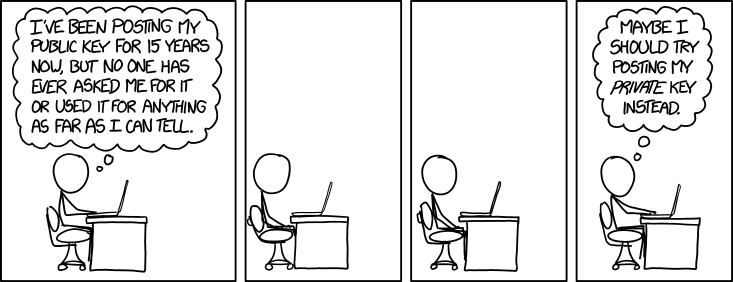
\includegraphics[width=0.75\textwidth]{Photos/Diffie_Hellman.png}
\end{center}

	\mysection{1}{Introduction to Diffie Hellman}
		Finally now we will study a public key cryptosystem in detail. Diffie and Hellman were some of the earliest cryptographers working to create a one-way trapdoor function - easy to compute, difficult to invert unless you have some trapdoor information.
		\begin{SCfigure}[0.5][h]
			\caption{Schematic of a trapdoor function}
			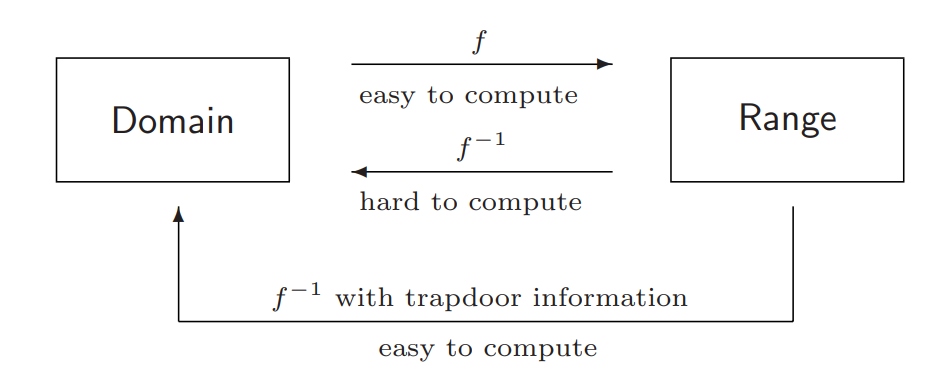
\includegraphics[width=0.6\textwidth]{Photos/DH_1.png}
		\end{SCfigure} 

		These functions are of a particular importance. As was explained in \textcolor{teal}{\hyperref[sec:asym]{Asymmetric Ciphers}} section, we make sure of \(k_{public}, \; e_k()\) for encryption which is made public knowledge whereas \(k_{private},\; d_k()\) are kept private as they are used for decryption. Since \(k_{public}\) is constructed from \(k_{private}\), it is important that the function that decides their relation is unidirectional else finding \(k_{private}\) will be possible for \(Eve\) from just the information that is publically available.

		\begin{mybox}
			\textbf{Why exactly is the use of public key cryptography even?}
			\tcblower
			Banks in the internet age would require to hand deliver keys to their clients which would massively slow down communications and created massive weaknesses in the line of communication. Hence finding a solution to this problem was important.
		\end{mybox}

		\quad But another thing to keep in mind is that if \(Bob\) is receiving the message from \(Alice\), he should be able to decrypt it since he has that extra information. \par

		Although ultimately Diffie and Hellman failed to create a public key cryptosystem (PKC), they did manage to create a system that can securely transfer certain data by utilising the Discrete Logarithm problem.

	\mysection{2}{Discrete Logarithm}
		Refer to \textcolor{teal}{\hyperref[sec:prime]{Prime numbers and Finite Fields}} for the background information in this section. According to the \textcolor{teal}{\hyperref[subsec:primitive]{Primitive Roots Theorem}}, in every \(\mathbb{F}_p\), there exists a \(g\) such that \(1, g^1, g^2, \ldots , g^{p-1}\) contains all the elements present in \(\mathbb{F}_p*\) and \(g^{p-1}\equiv 1 \bmod(p)\) (\textcolor{teal}{\hyperref[sec:fermat]{Fermat's Little Theorem}}).\par
		\emph{Discrete Logarithm Problem} (DLP) is the problem of finding \(x\) such that- \[g^x \equiv h \bmod(p)\] for some arbitrary \(h\) and \(x\) is called the \emph{discrete logarithm of h to the base g} \(= \log_g{h}\).\par
		\begin{mybox}
			\[x= \log_g{h} \bmod(p)= \text{Discrete logarithm(} h \text{)} \quad \text{for } x, h \in \mathbb{F}_p^*\]
		\end{mybox}
		\begin{tcolorbox}
			\textbf{\underline{Note-}} We use the term ``index'' to sometimes refer to the discrete logarithm i.e. \(x=\text{ind}_g{(h)}\). This is to ensure that the usual log and discrete log are not confused for each other.
		\end{tcolorbox}
		\(x' = x + (p-1) k \) would also satisfy our condition thus giving up \(\infty\)ly many solutions $x$. Hence \(x\) is only defined modulo (p-1). Hence we say that \[\text{ind}_g : \mathbb{F}_p* \rightarrow (\mathbb{Z}/(p-1)\mathbb{Z})\]
		\subsection{Why is it called logarithm?}
		Well you can easily see that \[\text{ind}_g (ab)=\text{ind}_g (a)+\text{ind}_g (b)\] and that gives us enough of a reason to call it so.

		\begin{tcolorbox}[breakable, title=Illustration,colback=brown!5!white,colframe=brown!75!black,colbacktitle=yellow!50!red,coltitle=red!25!black,fonttitle=\bfseries,subtitle style={boxrule=0.4pt,colback=yellow!50!red!25!white} ]
			If our prime number \(p = 56509\), and we know with surety that \(g = 2\) is a primitive root modulo \(p\), we can be sure that \(2\) is a ``generator'' of (\(\mathbb{Z} / p \mathbb{Z}*\)) hence the discrete logarithm of every number \(< p\) to the base \(2\) exists.

			In that case, if we have to calculate \(\text{ind}_2{38679}\), we will have to cycle through \textbf{every} one of \(1,2,2^2, 2^3, \cdots 2^{56508} \bmod(56509)\), until we get a value that matches \(38679\). This is exactly why the discrete logarithm problem is a formidable one.
			
			\tcbsubtitle{How did we know that 2 is a primitive root modulo 56509?}
				If we wanted to check if a number \(a\) is a primitive root modulo \(p\), the first approach that comes to mind might be to first evaluate all powers of \(a\) modulo \(p\) from 0 to \(p-2\) and see if all numbers from 1 to \(p-1\) appear exactly once. But this is too resource consuming so we use a better approach. 
				Since we know that if \(a\) is really a primitive root, then all the powers of \(a\) modulo \(p\) would be a bijective function with the set \({1, 2, 3, \cdots, p-1}\), we can be sure that 1 would appear once in the powers other than the \(p-1\)th power. (If 1 does not appear even once in between 0 and \(p-1\), we can be sure that all the values will \textbf{have} to be unique hence making \(a\) a primitive root).
				So we have \[a^{p-1} \equiv 1 \bmod(p)\] So we just have to calculate the prime factors (\(q_1, q_2, ...\)) of \(p-1\) and if 
				\[a^{\frac{p-1}{q_i}}\not \equiv 1 \bmod(p) \quad \forall i \text{ such that } q_i \text{ divides } p-1 \Rightarrow a \text{ is a primitive root modulo } p\] 

			\tcbsubtitle{Is it necessary for \(g\) to always be a primitive root modulo p?}
				No. As long as 2 things are ensured, we can always write \(\text{ind}_g{h}\)-
				\begin{enumerate}
					\item The discrete logarithm exists. \\e.g. In \hyperref[example:six]{this example}, \(\text{ind}_62\) is just not defined.
					\item The value is unique (in ring \(\mathbb{Z}/ p \mathbb{Z}\)) \\ e.g. In the \hyperref[example:six]{same example}, we can see that \(\text{ind}_66\) will have multiple values (1, 3, 5).
				\end{enumerate}
		\end{tcolorbox}

		The strongest point of our encryption using Discrete Logarithm is that there is a lot of variation and a seeming randomness in the values of the discrete logarithms in our data.
		\begin{SCfigure}[0.5][h]
			\caption{Table of values of \(h\) for \(g = 627\) and \(h= 941\)}
			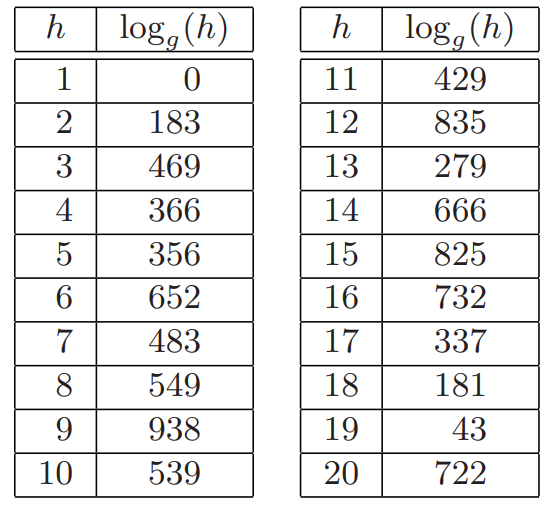
\includegraphics[width=0.4\textwidth]{Photos/Discrete_log_1.png}
		\end{SCfigure}

	\mysection{3}{Using Discrete Logarithm for Key Exchange}
		Let us say that \emph{Bob} and \emph{ALice} want to begin communication across an insecure channel. If they can agree upon a key, the communication can begin smoothly using any of the block or stream cipher ways we have already discussed. But how do you send the key, very well knowing that any and all information across the channel can easily get intercepted? \par
		In that case, \emph{Bob} and \emph{Alice} publicly agree upon \(g\) and \(p\). \emph{Alice} and \emph{Bob} then privately construct some \(a\) and \(b\) respectively without letting it be known to the outside world. \par
		\emph{Bob} then sends \emph{Alice} \(A = g^a \bmod(p)\) and \emph{Alice} sends back \(B = g^b \bmod(p)\). Due to the nature of the insecure channel, \emph{Eve} is able to safely intercept both \(A\) and \(B\). \par
		Finally \emph{Alice} calculates \(B^a \bmod(p)\) and \emph{Bob} calculates \(A^b \bmod(p)\). It is obvious that even in \(\mathbb{F}_p\), \(A^b = g^{ab} = B^a \bmod(p)\) hence that becomes the key the both parties use for secure communication henceforth.
		\emph{Eve}, despite knowing \(A, B, g\) and \(p\), is still unable to calculate \(g^{ab} \bmod(p)\) trivially because of her not knowing the values \(a\) and \(b\).

		\begin{center}
			\begin{tabular}{ c | c | c}
				 \hline
				 Information \emph{Bob} has & Information \emph{Alice} has & Information \emph{Eve} has\\ 
				 \hline
				 \hline
				 \multicolumn{3}{c}{\textbf{Before exchange}}\\
				 \hline
				 \(b,\; g,\; p,\; B\; (=g^b \bmod(p))\) & \(a,\; g,\; p,\; A\; (=g^a \bmod(p))\) & \(g,\; p\) \\
				 \hline
				 \multicolumn{3}{c}{\textbf{After exchange}}\\
				 \hline  
				 \(b,\; g,\; p,\; B,\; A\) & \(a,\; g,\; p,\; A,\; B\) & \(g,\; p,\; A,\; B\) \\
				 \multicolumn{2}{c}{Key (=\(A^b = B^a =g^{ab}\))} & No information about the key
			\end{tabular}
			\end{center}

		\begin{tcolorbox}[breakable, title=Does this mean that finding the key is a Discrete Logarithm Problem (DLP)?,colback=red!5!white,colframe=red!75!black]
			No. \\
			If the only way for \emph{Eve} to find the key was to find out \(a\) from \(A\) and \(g, p\) (or similarly \(b\) from \(B\) and \(g , p\)), then admittedly, this problem would have been a classic DLP problem.\par However, \emph{Eve} actually has both \(A\) and \(B\) and thus actually has to find \(g^{ab}\) using \(g^a\) and \(g^b\) which is definitely a simpler problem. This problem is termed as the \textbf{Diffle Hellman Problem} (DHP) and is not harder than the DLP.
			\tcblower
			We called DHP to be ``not more difficult than'' DLP instead of saying DHP is easier than DLP. The reason for it is that although we know if DLP was computable, DHP would be trivially solvable, the converse hasn't been proven.
		\end{tcolorbox}

		\begin{tcolorbox}
			For the modern standards of computing power, \(p\) needs to be \(\approx 1000\) bits for brute-force to not be a feasible option in \emph{Eve}`s hands. Also, \(g \approx p/2\) ensures most computational difficulty in the inversion of Discrete Logarithm.
		\end{tcolorbox}

		\centering{\Huge{\textcolor{orange}{But wait!}}} \par
		\raggedright \noindent Doesn't this mean we can effectively create a \emph{\hyperref[box:onetimepad]{One Time Pad}} (OTP) and hence an indecipherable means of communication is feasible using DHP? \\
		Yes, but also no.\footnote{At this point, the reader should just get used to seeing every question mark and brace themselves for a \hyperref[box:whyno]{heartless ``No.''}}\\
		Although it is very much possible to have a system wherein, 
		\begin{itemize}
			\item If \emph{Alice} and \emph{Bob} agree on only sharing 160-bit messages, they publicly choose a large enough (\(\approx 160\) bit)\(p, g\).
			\item Then both of them use \hyperref[subsec:prng]{PRNGs} privately to construct \(a, b\) of a suitable size so as to ensure that the final \(g^{ab}\) has a length larger than 160-bits.
			\item If the key has more than 160 bits, chop off the last few bits until you get a key \(k'\) of exactly 160 bit size.
			\item Use $\oplus$ (\text{xor}) on \(k'\) and \(m\) and then if \emph{Alice} sends this encrypted message to \emph{Bob}, \emph{Bob} can just calculate \(k' \oplus c \equiv m\) to get the original message.
			\item \emph{Alice} and \emph{Bob} change keys thus \(a\) and \(b\) for every message sent across the channel thus ensuring that they create a feasible One-Time Pad encrypted network.
		\end{itemize}

		\begin{mybox}\label{box:whyno}
			Although the above method is really great, it is not a secure system in today's times. The flaws this suffers from can best be explained at the \hyperref[sec:whydiffiesucks]{end of this chapter}.
		\end{mybox}

		\subsection{The anti-climactic conclusion of Diffie-Hellman}
			As you will come to see in the further sections, certain cases of Diffie Hellman are feasible to solve really quick and others can be solved with more efficient algorithms. There also exist some other flaws which prevent Diffie Hellman, despite all its glory, from becoming the cryptosystem standard it deserved to be. Rest in Peace :(

	\mysection{4}{ElGamal Public Key Cryptography}
		Fear not, for now we have a different approach to use the Discrete Logarithm Problem without having to sacrifice either speed or security (we don't want it to be any simpler to solve than the \textbf{DHP}).\\
		The steps for setting up an ElGamal Cryptosystem is as follows-
		\begin{enumerate}
			\item \emph{Alice} and \emph{Bob} agree on a \(g\) and a large enough \(p\).
			\item \emph{Alice} randomly\footnote{Of course, pseudo-randomly using a suitable \hyperref[subsec:prng]{PRNG} or such} chooses an \(a\) and publicly displays \(A \equiv g^a \bmod(p)\).
			\item \emph{Bob} then randomly\footnote{Again the same misnomer as above.} creates a \emph{ephemeral key} \(k\) (which will be used for this message only). 
			\item \emph{Bob} can only encrypt a message \(2< m < p\). He does so by calculating the 2 following values \(c_1 \equiv g^k \bmod(p)\) and \(c_2 \equiv m \cdot  A^k \bmod(p)\).
			\item He then sends \(c_1\) and \(c_2\) to \emph{Alice} who then can calculate \(m \equiv (c_1^a)^{-1} \cdot c_2 \bmod(p)\).
		\end{enumerate}

		\begin{mdframed}
			\centering \textbf{Proof of the above-}
			\[c_1^k \equiv g^{ak} \Rightarrow (c_1^k)^{-1} \equiv (g^{ak})^{-1} \bmod(p)\]
			\centering
				AND
			\[c_2 \equiv m \cdot (g^a)^k \equiv m \cdot g^{ak} \bmod(p)\]
			\raggedright Hence
			\[(c_1^a)^{-1} \cdot c_2 \bmod(p) \equiv (g^{ak})^{-1} \cdot m \cdot (g^{ak}) \equiv m \bmod(p)\]
		\end{mdframed}

		\begin{tcolorbox}[breakable, colback=blue!5!white,colframe=blue!75!black]
			Since \(c_1\) and \(c_2\) are of the same range of bits as \(m\), in order to send one bit of data, we send 2 bits of encrypted bits hence it is called a \emph{2-to-1 message expansion}.
		\end{tcolorbox}

		ElGamal Cryptography is as secure as the Diffie Hellman problem - i.e. in order to decrypt a ElGamal encrypted code, you need to solve the Diffie Hellman problem.\footnote{An intuitive proof would be- assume you have a machine that can decrypt any ElGamal encrypted data if you supplied it the necessary \(c_1\) and \(c_2\). In that case, providing \(c_1 = B\) and \(c_2 = 1\) just gives us \((c_1^a)^{-1}\cdot c_2 \equiv (g^{ab})^{-1} \bmod(p)\) hence giving us the Diffie Hellman key essentially.}

	\begin{mdframed}
	\mysection{5}{Mathematical Pre-requisite: Group Theory}
		\subsection{General properties of a Group}
			A group consists of a set $\mathbf{G}$ and a rule, which we denote by \(\star\), for combining two elements $a,b \in \mathbf{G}$ to obtain an element \(a\star b \in \mathbf{G}\). The composition operation \(\star\) is required to have the following three properties:
			\begin{itemize}
				\item \textbf{Identity law-} There exists an \(e \in \mathbf{G}\) such that, for every \(a \in \mathbf{G}\), \[a\star e = e \star a= a\]
				\item \textbf{Inverse law-} There exists a unique \(a^{-1} \in \mathbf{G}\) for every \(a \in \mathbf{G}\) such that, \[a \star a^{-1}= a^{-1} \star a = e\]
				\item \textbf{Associative law-} For every \(a, b, c \in \mathbf{G}\), \[a\star(b\star c )=(a\star b)\star c\]
				\item \textbf{Commutative law-} (optional- if group follows this as well, it is called a \emph{Commutative} or \emph{Abelian Group}) For every \(a, b \in \mathbf{G}\), \[a\star b = b \star a\] 
			\end{itemize}
			
			\begin{tcolorbox}
				Order of a group
				\tcblower
				\(|\mathbf{G}|\) or \(\# \mathbf{G}\) is the \emph{order of group \(\mathbf{G}\)} and it is the number of elements present in \(\mathbf{G}\). \(\mathbf{G}\) is called a \emph{finite group} if \(\# \mathbf{G} \in \text{finite} \mathbb{N}\). 
			\end{tcolorbox}

			\textbf{Examples-}
			\begin{enumerate}
				\item \(\mathbb{F}_p^*\) is a finite group, with order \((p-1)\) with composition operation \(\star = \times\) (multiplication). \(e=1\) and inverses do exist.
				\item \(\mathbb{Z}\) has \(\star = +\) (addition) and is an infinite group. \(e = 0\) and inverse of \(a \Rightarrow -a\)
				\item \(\mathbb{Z}\) with \(\star = \times\) is not a group since inverses do not exist inside the group for every element.
				\item A non commutative group can be \(\mathbf{G} = \begin{cases}\big(\begin{smallmatrix}
				  a & b\\ 
				  c & d
				\end{smallmatrix}\big)\end{cases} ; (ad-bc \not = 0)\). It has \(e = \big(\begin{smallmatrix}
				  1 & 0\\ 
				  0 & 1
				\end{smallmatrix}\big)\) and since \(\text{det}(A) \not = 0\) where \(A \) is a matrix \(\in \mathbf{G}\), an inverse also exists.
			\end{enumerate}

			If \(g\) is an element of \(\mathbf{G}\), \(g^x\) denotes \[\underbrace{g\star g\star g\star \cdots \star g}_{\text{x times}}\]
			\begin{itemize}
				\item[\(\#\)] \(g^0 = e\)
				\item[\(\#\)] If \(x<0\), we define \(g^x\) as \((g^{-1})^{|x|}\)
				\item[\(\#\)] Even though it may seem non-intuitive, \(g^x\) for \(\begin{cases}\mathbf{G}= \mathbb{Z}\\ \star=+ \end{cases}\) is actually \(g+ g+ g+ \cdots=x\cdot g\)
			\end{itemize}

			\begin{mybox}
				If \(a\in \mathbf{G}\), and if \(d\) is the smallest positive integer such that, \[a^d=e\] then \(d\) is called \textbf{order of a}. If no such \(d\) exists, \(a\) is said to have \textbf{infinite order}.
			\end{mybox}

			\subsection{Generalisation of Fermat's ``Little'' Theorem}
				
				If \(\mathbf{G}\) is a finite group, then every element \(\in \mathbf{G}\) will have finite order. \\ Furthermore, if \(a \in\mathbf{G}\) and has order \(d\), and\footnote{Trivial proof: Since \(d\) is the smallest positive integer which ensures \(a^d=e\), if we wrote \(k=q\cdot d + r\), where \(0<r<d\), then obviously \(a^k \not = e\)} \[a^k = e\Rightarrow d\;|\;k\]
			
			\begin{tcolorbox}[title=Lagrange's Theorem,colback=green!5!white,colframe=green!75!black]\label{theo:LagrangeTheo}
				Let \(\mathbf{G}\) be a finite group and let \(a \in \mathbf{G}\). Then the order of $a$ divides the order \(\mathbf{G}\).\footnote{Proof: If \(a\in\mathbf{G}=\{g_1, g_2, g_3, \cdots, g_n\}\), we can construct a new group \(\mathbf{S_a}=\{a\star g_1, a\star g_2, \cdots, a\star g_n\}\). Now using the definition of group (If \(a, b\in \mathbf{G}\), \(a\star b \in \mathbf{G}\) as well) we can be sure that every element of \(\mathbf{S_a}\) is an element of \(\mathbf{G}\) as well since \(a \in \mathbf{G}\). Keeping that in mind, \[a\star g_1 \times a\star g_2 \times \cdots \times a\star g_n = g_1 \times g_2 \times \cdots \times g_n\] Now we assume our group is Commutative (more general proof is slightly more rigorous) hence we can say that \[a^n = e\]}
				\tcblower
				\normalsize In other words, if \(|\mathbf{G}|=n\), then \[a^n=e \text{ AND } d\;|\;n\]
			\end{tcolorbox}
	\end{mdframed}

	\mysection{5}{How difficult is the DLP?}
		Up until now, we have claimed that the DLP is a very difficult problem. Now it is time to quantify the difficulty using big-\(\mathcal{O}\) notation.

		\subsection{Big- \(\mathcal{O}\) notation}
			\begin{tcolorbox}
				\textbf{Formal definition.} If $f(x)$ and $g(x)$ are 2 positive functions, $f(x)$ is called ``big-\(\mathcal{O}\) of $g(x)$'' iff there exists a positive $C,\; k$ such that \[|f(x)|\leq C\cdot |g(x)| \forall x>k\]
				\tcblower
				In other words, $f(x)= \mathcal{O}(g(x))$ iff \[\lim_{x\to\infty} \bigg|\frac{f(x)}{g(x)}\bigg|\text{ exists and is finite}\] 
			\end{tcolorbox}

			\textbf{\underline{Some examples}}-
			\begin{itemize}
				\item \(x^2 + 3x + 2981= \mathcal{O}(x^2)\)
				\item \((\log x)^{375} = \mathcal{O}(x^{0.001})\)
				\item \(x^2 \cdot 2^x= \mathcal{O}(e^x)\)
			\end{itemize}

			Although this is the mathematically pure definition, we will use a slightly different definition somewhat loosely while we talk of difficulty in the proceeding sections -

			\begin{mybox}
				\textbf{``Definition''.} If we made a proper list of ``complexities'' ($0, 1, \log n, n, n^2, n^3, \ldots 2^n, \ldots, n!, n^n\ldots$), and if \(f(x) = \mathcal{O}(g(x))\),  \(g(x)\) has to be the ``least complex'' function which satisfies the previous formal definition.
				\tcblower
				In other words, $f(x)= \mathcal{O}(g(x))$ iff \[\lim_{x\to\infty} \bigg|\frac{f(x)}{g(x)}\bigg|\text{ exists and is \textcolor{red}{non-zero} finite}\]
			\end{mybox}

			If an algorithm has an input of \(k\)-bits, then if output has order-
			\begin{itemize}
				\item[--] \(\mathcal{O}(k^a)\) where \(a \in \text{positive constant}\): Polynomial order \(\to\) ``Easy'' Problems
				\item[--] \(\mathcal{O}(e^{ax})\) where \(a \in \text{positive constant}\): Exponential order \(\to\) ``Hard'' Problems 
				\item[$\#$] There also exists a ``Sub-exponential order'' can be best described as ``grows faster than any polynomial function but slower than \textbf{any} exponential function of the form \(b^x \quad\forall b>1\).''
			\end{itemize}

		\subsection{Computing \(\mathcal{O}\) for DLP}
			\[g^x=h \text{ where }g\in\mathbf{G}=\mathbb{F}_{p}^{\ast} \text{ and } \star= \times \Rrightarrow \text{Finding \(x\), given \(g, p, h\)} \quad \cdots (\text{DLP})\]
			If \(p \in (2^k, 2^{k+1})\), then obviously \(p, g, h\) all will take individually \(k\)-bits at most. Thus we can say that input/data we are dealing with is \(\mathcal{O}(k)\).\par
			Using trial-and-error method, we will, in the worst case scenario, be evaulating all of the \((p-1)\) numbers from \(1\) to \(p-1\) hence order\( =\mathcal{O}(p)= \mathcal{O}(2^k)\) hence exponential \(\rightarrow\) \textcolor{red}{difficult}.\par
			But that is not the only approach we have in hand.
			\begin{itemize}
				\item[\(\ast\)] For some primes, where \(p-1\) can be factored into a product of small primes, we can use the \hyperref[sec:pohlig]{\emph{Pohlig-Hellman}} algorithm which makes the DLP for them quite \textcolor{red}{easy}.
				\item[\(\ast\)] \hyperref[sec:colli]{\emph{Collision algorithm}} works for all primes and takes \(\mathcal{O}(\sqrt{p} \log p)\) steps (still exponential but \textcolor{red}{easier than} \(\mathcal{O}(p)\))
				\item[\(\ast\)] Using index calculus, we can bring it down to \(\mathcal{O}(e^{c\sqrt{(\log p)( \log\log p )}})\) which is \textcolor{red}{sub-exponential}.
			\end{itemize}

		\subsection{How there is no inherent difficulty in DLP}
			The last few sections about DLP in \(\mathbb{F}_p^*\) might give you an impression that all DLPs of the form \(g^x = h \quad g, h\in \mathbf{G}\) are inherently difficult. \par
			In constrast, if \(\mathbf{G}=\mathbb{F}_p\) and \(\star = +\), our DLP can also be written as \[x \cdot g = h \bmod(p)\]
			Now using \hyperref[theo:extendedEuclid]{Extended Euclidean Theorem}, we know that finding \(g^{-1}\) in the above setup will take \(\mathcal{O}(\log p) = \mathcal{O}(\log 2^k)\) steps thus is solvable in \textcolor{red}{linear time}.

			With index calculus, DLP for \(\mathbf{G}=\mathbb{F}_p^*\) and \(\star=\times \) is solvable in \textcolor{red}{sub-exponential time}.

			If we instead had \emph{Elliptic curves}, our best algorithm for DLP takes \textcolor{red}{exponential time}.

	\mysection{6}{Collision Algorithm}\label{sec:colli}
		Collision Algorithms work by creating 2 lists, of approximately the same size for maximum efficiency and then comparing the 2 lists. This is considerably faster than just trial-and-error method we evaluated until now.

		\begin{tcolorbox}[breakable, title=Shank's ``Babystep- Giantstep'' Theorem,colback=blue!5!white,colframe=blue!75!black]
		 	Let \(g \in \mathbf{G}\) be an element of order \(N >2\). Then we can employ the following algorithm to get order of \(\mathcal{O}(\sqrt{N} \cdot \log N)\)\footnote{Proof: Making each list takes $n$ multiplications each (\hyperref[subsec:fastexpo]{fast powering algorithm}) and sorting and searching through the list takes another \(\mathcal{O}(\log n)\) steps- bringing the total time to \(\mathcal{O}(n \log n)= \mathcal{O}(\sqrt{N} \log N)\)}-
		 	\begin{enumerate}
		 		\item Let \(n = 1 + \lfloor\sqrt{N}\rfloor\) i.e. \(n> \sqrt{N}\).
		 		\item Then construct 2 lists- \[\text{List$_1$}= e, g, g^2, g^3, \ldots g^n\] \[\text{List$_2$}= h, h\cdot g^{-n}, h\cdot g^{-2n},
		 		\ldots , h\cdot g^{-n^2}\] 
		 		\item Now try to find the common entry in both lists. There should exist just one pair such that \[g^i = h \cdot g^{-j \times n}\]
		 		\item Then \(x = i + n \times j\) is the solution to \(g^x = h\).
		 	\end{enumerate}
		 \end{tcolorbox}
		 
		 \begin{mybox}
		 	\textbf{Intuitive explanation for how this works:} \\
		 	First of all, the size of \(\mathbf{G}\) does not matter since, if \(h\) is a valid solution of \(g^x = h\), \(x\) will have exactly one solution per \(N\) per values of $x$ we cycle through. We will only concentrate on the first \(N\) values i.e. the first \(x\) that satisfies our condition.\vspace{0.5cm}

		 	Moreover, we can write \(x= p \cdot n + q\) and since \(x\leq N \text{ AND } n>\sqrt{N}\text{, }p<\sqrt{N}\) and by remainder theorem, \(q<n\Rightarrow q<\sqrt{N}\). Hence if there was a way to make 2 lists such that one decides $p$ and the other sets $q$, our inversion algorithm would be successful.\vspace{0.5cm} 

		 	Hence we find \(u = (g^{-1})^n\) (which due to the \hyperref[theo:extendedEuclid]{extended Euclidean theorem}, is easy to compute) and then just find \(h, h\cdot u, h\cdot u^{2}, \ldots , h \cdot u^{n} \Rrightarrow \text{List}_2 \text{ a.k.a. $p$ setter}\). \(\text{List}_1\) is just \(e, g, g^2, \ldots, g^n\) which is the $q$ setter.\vspace{0.5cm}

		 	Finally when they correspond, \(h\cdot u^{p}=h\cdot (g^{-1})^{p\cdot n}= g^q \Rightarrow h = g^{p \cdot n + q}= g^x\)
		 \end{mybox} 
		 \begin{center}
		 	\Huge \textcolor{orange}{Jargon Overload}\\
		 	\normalsize That was a lot of jargon. Let's take a look at an example for better understanding.
		 \end{center}

		 \begin{tcolorbox}[breakable, title=Illustration,colback=brown!5!white,colframe=brown!75!black,colbacktitle=yellow!50!red,coltitle=red!25!black,fonttitle=\bfseries,subtitle style={boxrule=0.4pt,colback=yellow!50!red!25!white} ]
		 	In DLP, take \(\mathbf{G}=\mathbb{F}_p^*\) and \(\star=\times\) with \(p = 17389\), \(g= 9704\), and \(h=13896\). Find a suitable \(x\).
		 	\tcblower
		 	Order of \(g=9704\) in \(\mathbb{F}_{17389}^*\) is $1242$.\footnote{How did we get this order? \\The standard algorithm is to try and break \(17388\) into its prime factors and then try them one by one till the smallest factor \(k\) yields $g^k = e$. (Reason- Size of the group is 17388 hence using the \hyperref[theo:LagrangeTheo]{Langrange's Theorem}, we can be sure that the order is a factor of order of the group)}

		 	Using that, \[n = \lfloor\sqrt{N}\rfloor+1= 36\]
		 	Next, \[u=(9704^{-1})^{36}\]
		 	We find \(9704^{-1}\) using recursion with \hyperref[theo:extendedEuclid]{Extended Eucleadian Theorem} in linear time. After that, we just use \hyperref[subsec:fastexpo]{Fast Powering Algorithm} to find \(u\).\\
		 	That yields us \[u = 2494\]
		 	Now we constuct the two lists- 
		 	
		 	\begin{center}
		 		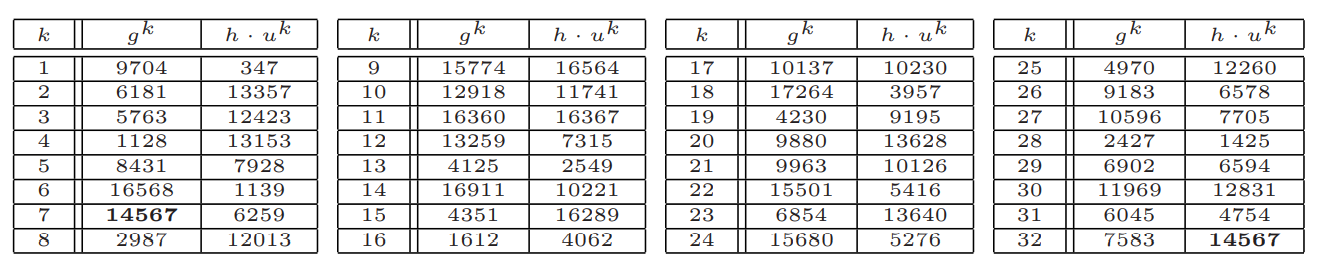
\includegraphics[width=0.8\textwidth]{Photos/DH_2.png}
		 	\end{center}

		 	As you can clearly see, \[9704^7=14567=13896 \cdot 2494^{32}= 13896 \cdot (9704^{-36})^{32}\Rightarrow13896= 9704^{1159}\Rightarrow x=1159\]
		 \end{tcolorbox}

	\mysection{7}{Congruences moduli composite numbers}
		Up until now, we have only dealt with congruences of the form \(\bmod(p); \: p \in \text{primes}\). But, what if we have to do computations in \(\bmod(m);\: m \not\in \text{primes}\)? Well that is where we get a helpful hand from the Chinese Remainder Theorem.
		
		\begin{mdframed}
			\subsection{Chinese Remainder Theorem}\label{subsec:chinese}
				Suppose you are given- \[x \equiv a \bmod(p) \text{ AND } x \equiv b \bmod(q) \text{; where $p$, $q\in $ primes}\]
				We can use this information to find the value of \textcolor{orange}{\(x \bmod(p\cdot q)\)}. 
				
				\textbf{Algorithm:}
				\begin{enumerate}
					\item Since \(x\equiv a \bmod(p)\), we can write \(x = a + p \cdot y\).
					\item Input that in the second congruence to get \(p \cdot y \equiv b -a \bmod(q)\). Now since \(\gcd(p,q)=1\) (prime numbers, duh), we know that \(p^{-1}\) exists.
					\item Hence finally we get \(y \equiv p^{-1}(b-a)\bmod(q)\)
					\item Assuming \(y<q\), we input the RHS into \(x= a + p \cdot y\) and viola! We just got a value of \(x\) in modulo \(p\cdot q\) (since, if \(c_1\) and \(c_2\) are solutions of \(x\) in this situation, \(c_1 = k\cdot (p\cdot q) + c_2\))
				\end{enumerate}
				\begin{tcolorbox}[breakable, title=Illustration,colback=brown!5!white,colframe=brown!75!black,colbacktitle=yellow!50!red,coltitle=red!25!black,fonttitle=\bfseries,subtitle style={boxrule=0.4pt,colback=yellow!50!red!25!white} ]
					\[x\equiv 1 \bmod(5) \text{ AND } x \equiv 9 \bmod(11)\]
					Thus \[x = 1 + 5 y\Rightarrow 5 y \equiv 8 \bmod(11)\]
					Now \(5^{-1}=9\). Using that, \[y \equiv 72 \bmod(11)\equiv 6 \bmod(11)\]
					Finally \(y =6 \Rightarrow x = 31\) is a particular solution. The final answer is-\[x\equiv 31 \bmod(55) \Leftrightarrow x = 31 + 55k \]
				\end{tcolorbox}

				Extending it to multiple numbers is just iteratively i.e. if \(\gcd(m_1, m_2, m_3, \ldots, m_i)=1\), \(x\equiv a_1\bmod(m_1)\), \(x\equiv a_2\bmod(m_2)\), \(x\equiv a_3\bmod(m_3)\), ... , \(x\equiv a_i\bmod(m_i)\). Now just try to find \(x \bmod(m_1\cdot m_2)\) and then continue accordingly since \(\gcd(m_1\cdot m_2, m_3)=1\).
		\end{mdframed}

		And thus we can just decompose any \(m\) into a product of primes and then apply Chinese Remainder Theorem. 

		\subsection{Application of CRT}			
			A good use\(\Rightarrow\) Finding square roots in modulo $m$. It is actually easy to calculate square roots in modulo prime, and more so in primes of form \(4l + 3\). \\ If \(x^2 \equiv a \bmod(p)\), then we can write that \(x\equiv a^\frac{p+1}{4} \bmod(p)\) \par
			How? Well, if we assumed \(g\) is the primitive root modulo \(p\), we can write \(x \equiv b \equiv g^k\) as a solution. Then, \[x^2 \equiv a^\frac{p+1}{2} \equiv a^\frac{p-1}{2} \cdot a \equiv g^{k \cdot (p-1)}\cdot a \equiv 1 \cdot a \bmod(p) \]
			Using this, if we had to solve for \(x^2 \equiv a \bmod(m)\) where \(m = p_1 \cdot p_2\), if they are of the form \(4\alpha +3\), we can easily write, \[x\text{ can be found by solving the congruences of $y$ and $z$} \text{ where } y^2 \equiv a \bmod(p_1)\text{ and } z^2 \equiv a \bmod(p_2)\] We can solve according to the previously discussed method. \par
			\textbf{Note:} \(x^2 \equiv a \bmod(p)\) will have 2 solutions but the above one will have 4 solutions since we can solve 4 different final congruences based on + - changes.
		\begin{mybox}
			Factorisation of \(m\) isn't really easy as \(m\) increases in size. In that case, directly evaluating whether or not the roots exist or not becomes really a tedious task. We can use that to construct a trapdoor function-  \href{https://bit.ly/3IFyTW7}{``Goldwasser–Micali'' Cryptosystems}\footnote{\cite{IIScGold}} depend on this function with the trapdoor information being the factors of \(m\).
		\end{mybox}

	\mysection{8}{Pohlig-Hellman Algorithm} \label{sec:pohlig}
		Pohlig-Hellman first starts off by analysing the fact that when we are talking about solutions of \(g^x \equiv h \bmod(p)\), \(x \in \mathbb{Z}/(p-1)\mathbb{Z}\) since \(x = p-1\) will just give the same value as \(x = 0\). So we try to exploit the fact that \(p-1\), an obviously composite number has prime roots and hodge podge a solution using \hyperref[subsec:chinese]{Chinese Remainder Theorem}.\par
		Let us first start off with an example instead of the actual theory. 

		\begin{tcolorbox}[breakable, title=Illustration,colback=brown!5!white,colframe=brown!75!black,colbacktitle=yellow!50!red,coltitle=red!25!black,fonttitle=\bfseries,subtitle style={boxrule=0.4pt,colback=yellow!50!red!25!white} ]
			
			Given that \(2\) is a generator of 211 (a.k.a. primitive root modulo 211), find \(x\) such that\footnote{Example was taken from \href{https://bit.ly/3O8XIKX}{this video}.} \[2^x \equiv 41 \bmod(211)\]
			\textbf{Proof:}\\
			Since we know that $2$ is a generator, we can be sure that a solution exists. Now, let us suspend belief for a few fleeting seconds and just find the roots of \(\phi(211)= 210\). The factorisation yields \(210 = 2\cdot 3\cdot 5\cdot 7\).\\
			Again, as a leap of faith just find \(a^\frac{\phi(p)}{7} \bmod(p)\) (for sake of simplicity, refer to \(211\) as $p$ and \(a \equiv 2^x \equiv 41\))
			\[a^\frac{\phi(p)}{7}\equiv (2^x)^\frac{\phi(p)}{7} \bmod(p) \]
			\[\text{Using remainder theorem, write } x=7q +r \Rightarrow 2^{q\cdot \phi(p)}\cdot 2^\frac{r\cdot\phi(p)}{7}\equiv 1\cdot 2^\frac{r\cdot\phi(p)}{7} \bmod(p)\]
			\[\text{Hence, } 41^\frac{\phi(p)}{7}\equiv 2^\frac{r\cdot\phi(p)}{7}\Rightarrow 41^{2\cdot 3\cdot 5}\equiv 2^{r\cdot 2 \cdot 3\cdot 5} \bmod(p)\]
			Now the funny thing is, since \(r<7\), we can just check all values of $r$ in \(\{0, 1, \ldots , 6\}\) to get finally, \(x\equiv 3 \bmod(7)\). \\~\\
			We do the same with 5 (run all values of $r$ from \(0\) to \(4\) in \(41^{2\cdot 3\cdot 7}\equiv 2^{r\cdot 2 \cdot 3\cdot 7} \bmod(p)\)) to get \(x\equiv 2 \bmod(5)\)\\~\\
			For 3 \(\Rightarrow x\equiv 2 \bmod(3)\)\\~\\
			For 2 \(\Rightarrow x \equiv 1 \bmod(2)\)\par
			Finally, we have 4 equations which we can stitch togther using Chinese Remainder theorem to get \[x\equiv 17 \bmod(210) \]
			Since $210<211$, we can safely say that any value we get this way is also the same for modulo 211 hence, \[2^{17} \equiv 41 \bmod(211)\]

		\end{tcolorbox}

		The power of \emph{Pohlig-Hellman Algorithm} lies in the fact that we need to apply trial-and-error only on small values of \(r\) (between 0 and the prime \(q_i\)) instead of from 1 to \(p-1\).

		\begin{tcolorbox}[breakable, title=Pohlig-Hellman Algorithm, colback=blue!5!white,colframe=blue!75!black]
			If \(g\in \mathbf{G}\) with an order of \(N\) and we can write \(N = q_1^{e_1}\cdot q_2^{e_2}\cdot \ldots \cdot q_m^{e_m}\) then we can solve the discrete lograrithm problem of the form \(g^x = h\) can be solved in \(\mathcal{O}(\sum^m_{i=1}S_{q_i^{e_i}}+ \log N)\) steps where \(S_{q_i^{e_i}} \) is the number of steps it takes to solve a discrete value problem in modulo \(q_i^{e_i}\) if we follow the algorithm.\\~\\
			In simpler words, if we are looking at the equation, \[g^x \equiv h \bmod(p)\] where \((p-1)\) can be factorised into \(q_1^{e_1}\cdot q_2^{e_2}\cdot \ldots \cdot q_m^{e_m}\), our problem can be solved using Pohlig-Hellman Algorithm in \(\mathcal{O}(\sum^m_{i=1}S_{q_i^{e_i}}+ \log N)\) steps where \(S_{q_i^{e_i}} \) is the number of steps it takes to solve the DLP
			\[ g^{\bigg\{r\cdot \big(\prod_{j\not = i}^{m}q_j^{e_j}\big)\bigg\}}\equiv g^{\big\{r\cdot \frac{(p-1)}{q_i^{e_i}}\big\}}\equiv h^{\big\{\frac{(p-1)}{q_i^{e_i}}\big\}} \bmod(p)\]
		\end{tcolorbox}

		We can further optimise the algorithm to get \(\mathcal{O}(e\cdot S_q)\). Using index calculus, we can cut it down further.

		\begin{tcolorbox}
			Pohlig-Hellman Algorithm illustrates that $p$ of the form \(p = 2 q + 1\), where \(q \in\) prime is the more secure in comparison to others.
		\end{tcolorbox}

	\mysection{9}{Why don't we use pure DHP or any DLP based cryptosystem?}\label{sec:whydiffiesucks}
		As discussed above, there do exist a lot of algorithms that can considerably bring down the computation time for inversion of the DHP. But even then, we can carefully select the primes numbers and construct a system that is difficult to invert.\par
		The main issue is a \textbf{lack of authentication}.\par
		If \emph{Alice} and \emph{Bob} are talking over an insecure network such that \emph{Eve} is not only able to intercept but also block direct communication between \emph{Alice} and \emph{Bob} between their conversation, she can use the following trick to get information out of both of them without ever even solving the DHP.

		\begin{tcolorbox}[title=Man in the Middle Attack, breakable, colback=yellow!5!white,colframe=yellow!75!black]
 			\emph{Eve} sets a \(e\) of her own. Since \(g, p\) are openly available, she can just send \(E\) to both \emph{Bob} and \emph{Alice} and now the key becomes \(A^e\) when talking with \emph{Alice} and \(B^e\) when talking to \emph{Bob}. However, if we were able to attach some sort of authentication method to our system, we can still use it.
		\end{tcolorbox}